\documentclass[../main.tex]{subfiles}

\begin{document}
\section{Beautification of Images by Generative Adversarial Networks}
%%%% General introduction
For millennia, philosophers have been arguing about the nature of beauty. Yet after all these years, we still cannot confidently claim to understand what beauty even \textit{is}. Furthermore, the fundamental question whether beauty is subjective or objective remains unsettled \parencite{sep-beauty}. In this paper, we will use state-of-the-art machine learning techniques to try and create a so-called `visual definition' of beauty.


%%%% Philosophy
\subsection{Defining Beauty}
% What is beauty?
Throughout history, there have been different conceptions of beauty. The classical conception of beauty, often embodied in classical art, typically concerns the arrangement of independent parts into a coherent whole through properties such as symmetry and order \parencite{wolfflin1932principles, sep-beauty}. Another important conception is the idealist conception of beauty described by Plato as a perfect unity. This is in contrast to the classical conception which emphasizes the composition of independent parts \parencite{sep-beauty}. 18th century empiricist philosophers on the other hand looked at beauty in a more instrumental, hedonistic sense. \textcite{hume2003treatise} for example argues that beauty exists to give pleasure and satisfaction to the soul.

% Subjectivity and objectivity
While most classical philosophers would have argued that beauty is a property of an object that exists outside the mind, Renaissance and later philosophers argue more for a combination of some objective properties with unique subjective appreciations \parencite{sartwell2017entanglements}. The assumption that there are indeed some objective properties to beauty allows us to examine what exactly it means for something to be beautiful.

% Philosophy of aesthetics



%%%% Psychology
\subsection{How we Perceive Beauty}
% Transition to psychology
The shift from a pure objective conception of beauty towards a more nuanced combination of objective properties with subjective perception preceded the start of psychology as an empirical science in the 19th century. Among these early psychologists a school of thought known as Gestalt psychology came to fruition in the early 20th century. The Gestalt psychologists created a framework of visual perception that emphasizes patterns and configurations rather than individual components \parencite{wagemansCenturyGestaltPsychology2012a}. Examples of classic perceptual grouping principles are proximity, color, shape, size, symmetry, and continuation \parencite{wertheimer1923laws, brooks2015traditional}. In the Gestalt framework, principles such as these are the building blocks for our visual system \parencite{wagemansCenturyGestaltPsychology2012a}.

% Studies on aesthetics
Later psychological research focusing on art and aesthetic appreciation has found that there are  certain principles that tend to evoke a certain aesthetic quality across cultures such as for example symmetry \parencite{bodeCrossculturalComparisonPreference2017}, order and complexity \parencite{vangeert2021order}, and figure-ground contrast \parencite{reberProcessingFluencyAesthetic2004}. Mirroring the progression in philosophy, modern views on aesthetics from neuroscience and experimental psychology support an interactionist interpretation of beauty: objects do contain intrinsic properties conveying beauty, but the final aesthetic appraisal comes from an interaction between these objective properties and a subjective observer \parencite{valenziseAdvancesChallengesComputational2022}.

% Processing fluency
One influential framework that incorporates the interactionist interpretation of beauty is that of processing fluency formulated by \textcite{reberProcessingFluencyAesthetic2004}. In this framework, the aesthetic experience is determined by the fluency with which a perceived object is processed. Processing fluency relies on an interaction of objective properties such as the principles from Gestalt psychology with subjective factors such as personal experiences and expectations.

% Refer to AestheticsNet



\subsection{Machine Learning and Beauty}
% Introduce Computational Aesthetics
One of the biggest technological advances in recent years is in the field of machine learning. This `Deep Learning Revolution' was sparked by the continuous efforts of researchers and engineers, the increasing availability of big data, and the boost in computing power \parencite{sejnowskiDeepLearningRevolution2018}. Because these networks have some organizational similarities to the human brain, they can potentially be used as a means to study obscure mental representations in humans \parencite{guoDeepLearningVisual2016, goetschalckx2021generative}. 

Computational aesthetics is defined as the research of human aesthetic decision making through computational methods \parencite{valenziseAdvancesChallengesComputational2022, hoenig2005defining}. As a result of the deep learning revolution, more and more types of artificial neural networks have become available to be used as a means to study human aesthetic behavior.

\begin{figure}[!h]
	\caption{Schematic Representation of a Typical GAN}
	\label{fig:gan-simple}
	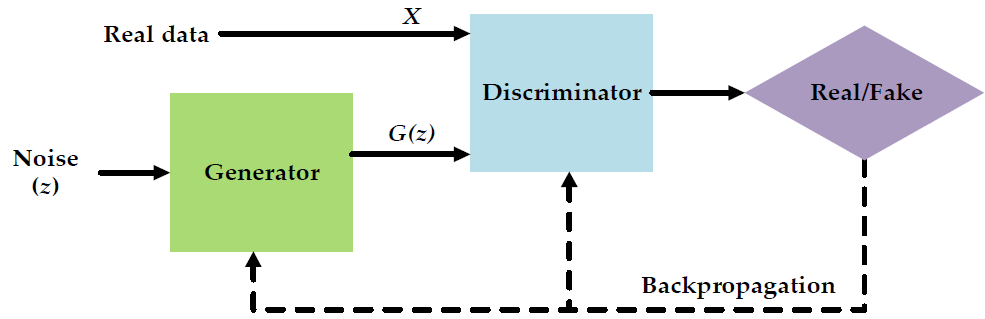
\includegraphics[width=1\linewidth]{images/gan_simple}
	{\textit{Note.} Reprinted from `Generative Adversarial Networks Based on Collaborative Learning and Attention Mechanism for Hyperspectral Image Classification', by Feng, J., Feng, X., Chen, J., Cao, X., Zhang, X., Jiao, L., \& Yu, T., 2020, \textit{Remote Sensing}, \textit{12}(7), p. 1152}
\end{figure}

% Introduction to GANs
Generative Adversarial Networks (GANs) are a relatively recent development characterized by two competing neural networks \parencite{goodfellow2014generative}. The purpose of a GAN is to learn the probability distribution of complex sensory data, allowing it to generate new sensory samples representative of the original dataset \parencite{goetschalckx2021generative}. In order to learn the probability distribution of a dataset consisting of images, a generator network with no access to the image dataset is used in combination with a discriminator network that does have access to this dataset \parencite{feng2020generative}. A schematic representation of how GANs typically work can be seen in Figure~\ref{fig:gan-simple}. Initially, the generator will output random pixel values that are then forwarded to the discriminator. The discriminator is then presented with two stimuli, either made by the generator or from the original dataset, with the task to select the image from the original dataset. Both networks then receive feedback: the generator learns that the generated image was not good enough to fool the discriminator, and the discriminator learns that it correctly identified the real image. For the next iteration, the generator will again attempt to produce an image but, as a result of the feedback, it has adjusted its internal weights resulting in an output that resembles the original dataset slightly better. Over time, both networks will improve at their respective tasks until the generator becomes so good at creating images that the discriminator is no longer able to reliably distinguish between real and fake.

% Use of GANs in cognitive science

% GANalyze to obtain a visual definition
\begin{figure}[!h]
	\caption{Schematic Representation of GANalyze}
	\label{fig:ganalyze}
	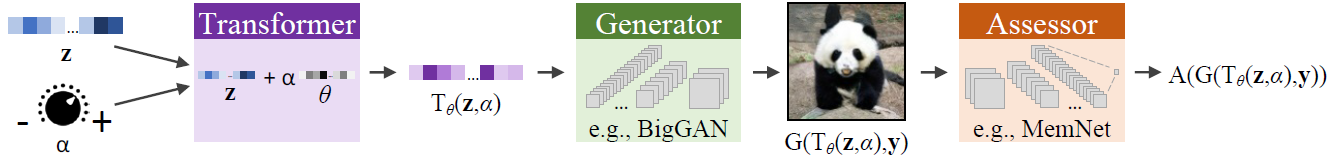
\includegraphics[width=1\linewidth]{images/ganalyze}
	{\textit{Note.} Reprinted from `GANalyze: Toward Visual Definitions of Cognitive Image Properties', by Goetschalckx, L., Andonian, A., \& Oliva, A., 2019, \textit{Proceedings of the IEEE/CVF International Conference on Computer Vision (ICCV)}, 10, p. 5745}
\end{figure}

\textcite{goetschalckxGANalyzeVisualDefinitions2019} have developed GANalyze, a framework using GANs that allows us to study cognitive properties by means of so-called visual definitions. In their paper, they utilized their network to generate images of varying levels of memorability which were validated in a behavioral task. GANalyze makes this possible by using as the discriminator a pretrained convolutional neural network (CNN) designed for predicting image memorability \parencite{khosla2015understanding}. A schematic representation of the GANalyze model can be seen in Figure~\ref{fig:ganalyze}. GANalyze is configured in such a way that instead of the generator learning weights to create images that resemble an existing dataset, it learns to adjust its weights to transform a random noise vector such that the cognitive property of interest (e.g., aesthetic value) either increases or decreases \parencite{goetschalckxGANalyzeVisualDefinitions2019}. This transformer function takes as input an $\alpha$-value to determine the magnitude of the transformation. As the discriminator is a network pretrained on evaluating image properties, it will over time train the generator to make more convincing transformations targeting the optimal image features for influencing the cognitive property of interest.

% refer to https://linkinghub.elsevier.com/retrieve/pii/S1364661321001534 for GAN explanation such at latent space etc


%%%% Theoretical framing of the research problem
\subsection{Present Study}
The goal of this study is to investigate the factors underlying the aesthetic value of images using GANalyze. We will use GANalyze to generate sequences of images that we hypothesize possess either \textit{more}, or \textit{less} aesthetic quality depending on the $\alpha$-value used for their respective generations. By comparing the low-aesthetic images to the high-aesthetic images, we will be able to examine the underlying factors responsible for making an image either more or less beautiful.

% AestheticNet & BigGAN potentially

% GANalyze validation
However, if we wish to learn something about human aesthetics appraisal from a GAN, we must first validate whether the GAN truly captures what it means for an image to possess aesthetic quality. To do so, we will validate whether human participants tend to agree with GANalyze on which image appears to be more beautiful. We are also interested whether a person's experience with art and their demographic characteristics affect their proportion of agreement with the GAN. A relation between art experience and agreement with the GAN could have important implications for the validation of the network and the generalizability of the final results.


\end{document}